\section{Wyznaczenie odpowiedzi skokowej toru zakłócenie-wyjście}
\label{lab:zad2}


-------POLECENIE--------

Wyznaczyc odpowiedzi skokowe toru zakłócenie-wyjscie procesu dla trzech róznych
zmian sygnału zakłócajacego Z rozpoczynajac z punktu pracy. Narysowac otrzymane
przebiegi na jednym rysunku. Czy własciwosci statyczne obiektu mozna okreslic jako
(w przyblizeniu) liniowe? Jezeli tak, okreslic wzmocnienie statyczne tego toru procesu.

-------POLECENIE--------

Odpowiedzi skokowe toru zakłócenie-wyjście zostały wyznaczone symulacyjnie dla pięciu
zmian sygnału zakłócenia .

\subsection{Odpowiedzi skokowe obiektu}
\label{lab:zad2:odpSkok}

Do uzyskania odpowiedzi skokowych dla tego toru ustawiono sygnał wejściowy na stałą
wartość U=32, 
przy ustabilizowanej temperaturze T1=35.4 stp C przeprowadzone zostały
skoki sterowania z Z =0 na 10, 15 oraz 30.

\begin{figure}[H] 
    \centering
    % This file was created by matlab2tikz.
%
\definecolor{mycolor1}{rgb}{0.00000,0.44700,0.74100}%
\definecolor{mycolor2}{rgb}{0.85000,0.32500,0.09800}%
\definecolor{mycolor3}{rgb}{0.92900,0.69400,0.12500}%
%
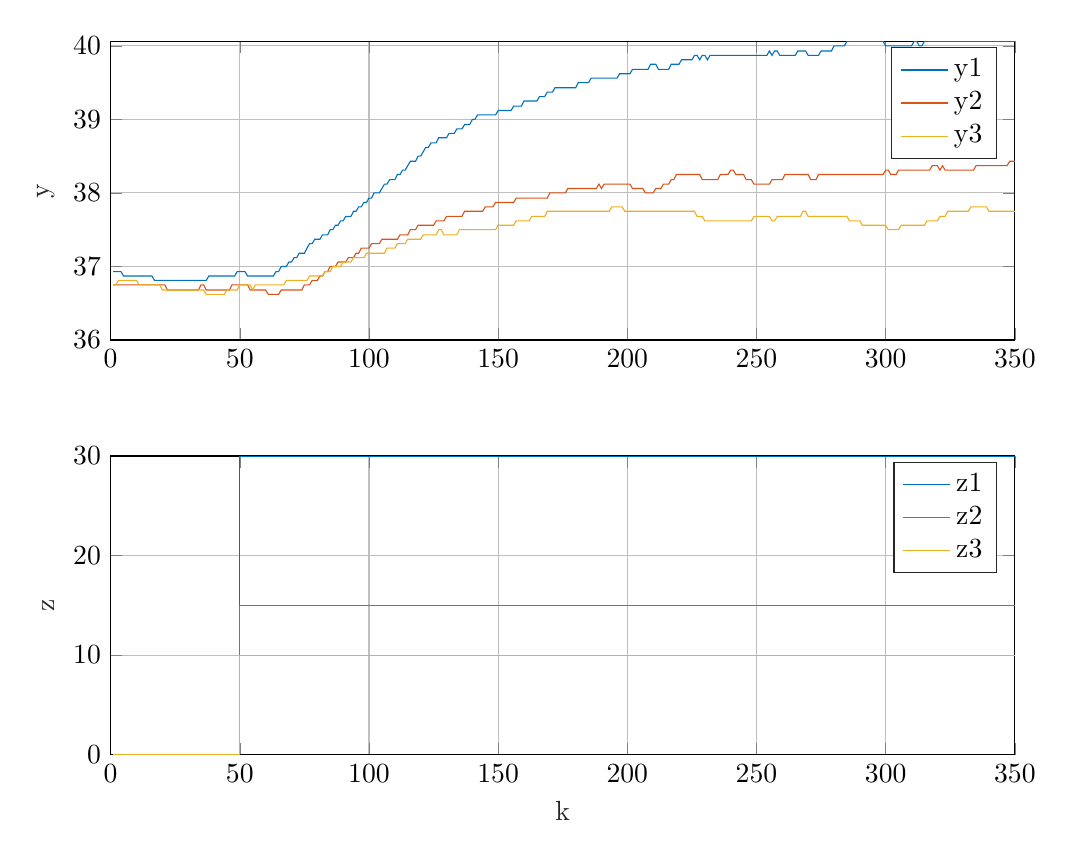
\begin{tikzpicture}

\begin{axis}[%
width=4.521in,
height=1.493in,
at={(0.758in,2.554in)},
scale only axis,
xmin=0,
xmax=350,
ymin=36,
ymax=40.06,
ylabel style={font=\color{white!15!black}},
ylabel={y},
axis background/.style={fill=white},
xmajorgrids,
ymajorgrids,
legend style={legend cell align=left, align=left, draw=white!15!black}
]
\addplot [color=mycolor1]
  table[row sep=crcr]{%
1	36.93\\
2	36.93\\
3	36.93\\
4	36.93\\
5	36.87\\
6	36.87\\
7	36.87\\
8	36.87\\
9	36.87\\
10	36.87\\
11	36.87\\
12	36.87\\
13	36.87\\
14	36.87\\
15	36.87\\
16	36.87\\
17	36.81\\
18	36.81\\
19	36.81\\
20	36.81\\
21	36.81\\
22	36.81\\
23	36.81\\
24	36.81\\
25	36.81\\
26	36.81\\
27	36.81\\
28	36.81\\
29	36.81\\
30	36.81\\
31	36.81\\
32	36.81\\
33	36.81\\
34	36.81\\
35	36.81\\
36	36.81\\
37	36.81\\
38	36.87\\
39	36.87\\
40	36.87\\
41	36.87\\
42	36.87\\
43	36.87\\
44	36.87\\
45	36.87\\
46	36.87\\
47	36.87\\
48	36.87\\
49	36.93\\
50	36.93\\
51	36.93\\
52	36.93\\
53	36.87\\
54	36.87\\
55	36.87\\
56	36.87\\
57	36.87\\
58	36.87\\
59	36.87\\
60	36.87\\
61	36.87\\
62	36.87\\
63	36.87\\
64	36.93\\
65	36.93\\
66	37\\
67	37\\
68	37\\
69	37.06\\
70	37.06\\
71	37.12\\
72	37.12\\
73	37.18\\
74	37.18\\
75	37.18\\
76	37.25\\
77	37.31\\
78	37.31\\
79	37.37\\
80	37.37\\
81	37.37\\
82	37.43\\
83	37.43\\
84	37.43\\
85	37.5\\
86	37.5\\
87	37.56\\
88	37.56\\
89	37.62\\
90	37.62\\
91	37.68\\
92	37.68\\
93	37.68\\
94	37.75\\
95	37.75\\
96	37.81\\
97	37.81\\
98	37.87\\
99	37.87\\
100	37.93\\
101	37.93\\
102	38\\
103	38\\
104	38\\
105	38.06\\
106	38.12\\
107	38.12\\
108	38.18\\
109	38.18\\
110	38.18\\
111	38.25\\
112	38.25\\
113	38.31\\
114	38.31\\
115	38.37\\
116	38.43\\
117	38.43\\
118	38.43\\
119	38.5\\
120	38.5\\
121	38.56\\
122	38.62\\
123	38.62\\
124	38.68\\
125	38.68\\
126	38.68\\
127	38.75\\
128	38.75\\
129	38.75\\
130	38.75\\
131	38.81\\
132	38.81\\
133	38.81\\
134	38.87\\
135	38.87\\
136	38.87\\
137	38.93\\
138	38.93\\
139	38.93\\
140	39\\
141	39\\
142	39.06\\
143	39.06\\
144	39.06\\
145	39.06\\
146	39.06\\
147	39.06\\
148	39.06\\
149	39.06\\
150	39.12\\
151	39.12\\
152	39.12\\
153	39.12\\
154	39.12\\
155	39.12\\
156	39.18\\
157	39.18\\
158	39.18\\
159	39.18\\
160	39.25\\
161	39.25\\
162	39.25\\
163	39.25\\
164	39.25\\
165	39.25\\
166	39.31\\
167	39.31\\
168	39.31\\
169	39.37\\
170	39.37\\
171	39.37\\
172	39.43\\
173	39.43\\
174	39.43\\
175	39.43\\
176	39.43\\
177	39.43\\
178	39.43\\
179	39.43\\
180	39.43\\
181	39.5\\
182	39.5\\
183	39.5\\
184	39.5\\
185	39.5\\
186	39.56\\
187	39.56\\
188	39.56\\
189	39.56\\
190	39.56\\
191	39.56\\
192	39.56\\
193	39.56\\
194	39.56\\
195	39.56\\
196	39.56\\
197	39.62\\
198	39.62\\
199	39.62\\
200	39.62\\
201	39.62\\
202	39.68\\
203	39.68\\
204	39.68\\
205	39.68\\
206	39.68\\
207	39.68\\
208	39.68\\
209	39.75\\
210	39.75\\
211	39.75\\
212	39.68\\
213	39.68\\
214	39.68\\
215	39.68\\
216	39.68\\
217	39.75\\
218	39.75\\
219	39.75\\
220	39.75\\
221	39.81\\
222	39.81\\
223	39.81\\
224	39.81\\
225	39.81\\
226	39.87\\
227	39.87\\
228	39.81\\
229	39.87\\
230	39.87\\
231	39.81\\
232	39.87\\
233	39.87\\
234	39.87\\
235	39.87\\
236	39.87\\
237	39.87\\
238	39.87\\
239	39.87\\
240	39.87\\
241	39.87\\
242	39.87\\
243	39.87\\
244	39.87\\
245	39.87\\
246	39.87\\
247	39.87\\
248	39.87\\
249	39.87\\
250	39.87\\
251	39.87\\
252	39.87\\
253	39.87\\
254	39.87\\
255	39.93\\
256	39.87\\
257	39.93\\
258	39.93\\
259	39.87\\
260	39.87\\
261	39.87\\
262	39.87\\
263	39.87\\
264	39.87\\
265	39.87\\
266	39.93\\
267	39.93\\
268	39.93\\
269	39.93\\
270	39.87\\
271	39.87\\
272	39.87\\
273	39.87\\
274	39.87\\
275	39.93\\
276	39.93\\
277	39.93\\
278	39.93\\
279	39.93\\
280	40\\
281	40\\
282	40\\
283	40\\
284	40\\
285	40.06\\
286	40.06\\
287	40.06\\
288	40.06\\
289	40.06\\
290	40.06\\
291	40.06\\
292	40.06\\
293	40.06\\
294	40.06\\
295	40.06\\
296	40.06\\
297	40.06\\
298	40.06\\
299	40.06\\
300	40\\
301	40\\
302	40\\
303	40\\
304	40\\
305	40\\
306	40\\
307	40\\
308	40\\
309	40\\
310	40\\
311	40.06\\
312	40.06\\
313	40\\
314	40\\
315	40.06\\
316	40.06\\
317	40.06\\
318	40.06\\
319	40.06\\
320	40.06\\
321	40.06\\
322	40.06\\
323	40.06\\
324	40.06\\
325	40.06\\
326	40.06\\
327	40.06\\
328	40.06\\
329	40.06\\
330	40.06\\
331	40.06\\
332	40.06\\
333	40.06\\
334	40.06\\
335	40.06\\
336	40.06\\
337	40.06\\
338	40.06\\
339	40.06\\
340	40.06\\
341	40.06\\
342	40.06\\
343	40.06\\
344	40.06\\
345	40.06\\
346	40.06\\
347	40.06\\
348	40.06\\
349	40.06\\
350	40.06\\
351	40.06\\
352	40.06\\
353	40.06\\
354	40.12\\
355	40.12\\
356	40.12\\
357	40.12\\
358	40.12\\
359	40.12\\
360	40.12\\
361	40.12\\
362	40.12\\
363	40.12\\
364	40.12\\
365	40.12\\
};
\addlegendentry{y1}

\addplot [color=mycolor2]
  table[row sep=crcr]{%
1	36.75\\
2	36.75\\
3	36.75\\
4	36.75\\
5	36.75\\
6	36.75\\
7	36.75\\
8	36.75\\
9	36.75\\
10	36.75\\
11	36.75\\
12	36.75\\
13	36.75\\
14	36.75\\
15	36.75\\
16	36.75\\
17	36.75\\
18	36.75\\
19	36.75\\
20	36.75\\
21	36.75\\
22	36.68\\
23	36.68\\
24	36.68\\
25	36.68\\
26	36.68\\
27	36.68\\
28	36.68\\
29	36.68\\
30	36.68\\
31	36.68\\
32	36.68\\
33	36.68\\
34	36.68\\
35	36.75\\
36	36.75\\
37	36.68\\
38	36.68\\
39	36.68\\
40	36.68\\
41	36.68\\
42	36.68\\
43	36.68\\
44	36.68\\
45	36.68\\
46	36.68\\
47	36.75\\
48	36.75\\
49	36.75\\
50	36.75\\
51	36.75\\
52	36.75\\
53	36.75\\
54	36.68\\
55	36.68\\
56	36.68\\
57	36.68\\
58	36.68\\
59	36.68\\
60	36.68\\
61	36.62\\
62	36.62\\
63	36.62\\
64	36.62\\
65	36.62\\
66	36.68\\
67	36.68\\
68	36.68\\
69	36.68\\
70	36.68\\
71	36.68\\
72	36.68\\
73	36.68\\
74	36.68\\
75	36.75\\
76	36.75\\
77	36.75\\
78	36.81\\
79	36.81\\
80	36.81\\
81	36.87\\
82	36.87\\
83	36.93\\
84	36.93\\
85	37\\
86	37\\
87	37\\
88	37.06\\
89	37.06\\
90	37.06\\
91	37.06\\
92	37.12\\
93	37.12\\
94	37.12\\
95	37.18\\
96	37.18\\
97	37.25\\
98	37.25\\
99	37.25\\
100	37.25\\
101	37.31\\
102	37.31\\
103	37.31\\
104	37.31\\
105	37.37\\
106	37.37\\
107	37.37\\
108	37.37\\
109	37.37\\
110	37.37\\
111	37.37\\
112	37.43\\
113	37.43\\
114	37.43\\
115	37.43\\
116	37.5\\
117	37.5\\
118	37.5\\
119	37.56\\
120	37.56\\
121	37.56\\
122	37.56\\
123	37.56\\
124	37.56\\
125	37.56\\
126	37.62\\
127	37.62\\
128	37.62\\
129	37.62\\
130	37.68\\
131	37.68\\
132	37.68\\
133	37.68\\
134	37.68\\
135	37.68\\
136	37.68\\
137	37.75\\
138	37.75\\
139	37.75\\
140	37.75\\
141	37.75\\
142	37.75\\
143	37.75\\
144	37.75\\
145	37.81\\
146	37.81\\
147	37.81\\
148	37.81\\
149	37.87\\
150	37.87\\
151	37.87\\
152	37.87\\
153	37.87\\
154	37.87\\
155	37.87\\
156	37.87\\
157	37.93\\
158	37.93\\
159	37.93\\
160	37.93\\
161	37.93\\
162	37.93\\
163	37.93\\
164	37.93\\
165	37.93\\
166	37.93\\
167	37.93\\
168	37.93\\
169	37.93\\
170	38\\
171	38\\
172	38\\
173	38\\
174	38\\
175	38\\
176	38\\
177	38.06\\
178	38.06\\
179	38.06\\
180	38.06\\
181	38.06\\
182	38.06\\
183	38.06\\
184	38.06\\
185	38.06\\
186	38.06\\
187	38.06\\
188	38.06\\
189	38.12\\
190	38.06\\
191	38.12\\
192	38.12\\
193	38.12\\
194	38.12\\
195	38.12\\
196	38.12\\
197	38.12\\
198	38.12\\
199	38.12\\
200	38.12\\
201	38.12\\
202	38.06\\
203	38.06\\
204	38.06\\
205	38.06\\
206	38.06\\
207	38\\
208	38\\
209	38\\
210	38\\
211	38.06\\
212	38.06\\
213	38.06\\
214	38.12\\
215	38.12\\
216	38.12\\
217	38.18\\
218	38.18\\
219	38.25\\
220	38.25\\
221	38.25\\
222	38.25\\
223	38.25\\
224	38.25\\
225	38.25\\
226	38.25\\
227	38.25\\
228	38.25\\
229	38.18\\
230	38.18\\
231	38.18\\
232	38.18\\
233	38.18\\
234	38.18\\
235	38.18\\
236	38.25\\
237	38.25\\
238	38.25\\
239	38.25\\
240	38.31\\
241	38.31\\
242	38.25\\
243	38.25\\
244	38.25\\
245	38.25\\
246	38.18\\
247	38.18\\
248	38.18\\
249	38.12\\
250	38.12\\
251	38.12\\
252	38.12\\
253	38.12\\
254	38.12\\
255	38.12\\
256	38.18\\
257	38.18\\
258	38.18\\
259	38.18\\
260	38.18\\
261	38.25\\
262	38.25\\
263	38.25\\
264	38.25\\
265	38.25\\
266	38.25\\
267	38.25\\
268	38.25\\
269	38.25\\
270	38.25\\
271	38.18\\
272	38.18\\
273	38.18\\
274	38.25\\
275	38.25\\
276	38.25\\
277	38.25\\
278	38.25\\
279	38.25\\
280	38.25\\
281	38.25\\
282	38.25\\
283	38.25\\
284	38.25\\
285	38.25\\
286	38.25\\
287	38.25\\
288	38.25\\
289	38.25\\
290	38.25\\
291	38.25\\
292	38.25\\
293	38.25\\
294	38.25\\
295	38.25\\
296	38.25\\
297	38.25\\
298	38.25\\
299	38.25\\
300	38.31\\
301	38.31\\
302	38.25\\
303	38.25\\
304	38.25\\
305	38.31\\
306	38.31\\
307	38.31\\
308	38.31\\
309	38.31\\
310	38.31\\
311	38.31\\
312	38.31\\
313	38.31\\
314	38.31\\
315	38.31\\
316	38.31\\
317	38.31\\
318	38.37\\
319	38.37\\
320	38.37\\
321	38.31\\
322	38.37\\
323	38.31\\
324	38.31\\
325	38.31\\
326	38.31\\
327	38.31\\
328	38.31\\
329	38.31\\
330	38.31\\
331	38.31\\
332	38.31\\
333	38.31\\
334	38.31\\
335	38.37\\
336	38.37\\
337	38.37\\
338	38.37\\
339	38.37\\
340	38.37\\
341	38.37\\
342	38.37\\
343	38.37\\
344	38.37\\
345	38.37\\
346	38.37\\
347	38.37\\
348	38.43\\
349	38.43\\
350	38.43\\
351	38.43\\
352	38.43\\
353	38.43\\
354	38.43\\
355	38.43\\
356	38.43\\
357	38.43\\
358	38.43\\
359	38.43\\
360	38.43\\
361	38.43\\
362	38.43\\
363	38.43\\
364	38.43\\
365	38.43\\
366	38.43\\
367	38.43\\
368	38.43\\
369	38.43\\
370	38.37\\
371	38.37\\
372	38.37\\
373	38.43\\
374	38.43\\
375	38.5\\
376	38.5\\
377	38.5\\
378	38.5\\
379	38.56\\
380	38.56\\
381	38.56\\
382	38.56\\
383	38.56\\
384	38.56\\
385	38.56\\
386	38.56\\
387	38.5\\
388	38.5\\
389	38.56\\
390	38.56\\
391	38.56\\
392	38.5\\
393	38.5\\
394	38.5\\
395	38.5\\
396	38.43\\
397	38.43\\
398	38.43\\
399	38.43\\
400	38.43\\
401	38.37\\
402	38.37\\
403	38.37\\
404	38.31\\
405	38.31\\
406	38.31\\
407	38.31\\
408	38.31\\
409	38.31\\
410	38.31\\
411	38.37\\
412	38.37\\
413	38.37\\
414	38.37\\
415	38.37\\
416	38.37\\
417	38.31\\
418	38.31\\
419	38.31\\
420	38.31\\
421	38.31\\
422	38.31\\
423	38.31\\
424	38.31\\
425	38.31\\
426	38.31\\
427	38.31\\
428	38.37\\
429	38.37\\
430	38.37\\
431	38.37\\
432	38.37\\
433	38.37\\
434	38.37\\
435	38.37\\
436	38.37\\
437	38.37\\
438	38.37\\
439	38.37\\
440	38.37\\
441	38.37\\
442	38.37\\
443	38.37\\
444	38.37\\
445	38.37\\
446	38.37\\
447	38.37\\
448	38.37\\
449	38.37\\
450	38.43\\
};
\addlegendentry{y2}

\addplot [color=mycolor3]
  table[row sep=crcr]{%
1	36.75\\
2	36.75\\
3	36.81\\
4	36.81\\
5	36.81\\
6	36.81\\
7	36.81\\
8	36.81\\
9	36.81\\
10	36.81\\
11	36.75\\
12	36.75\\
13	36.75\\
14	36.75\\
15	36.75\\
16	36.75\\
17	36.75\\
18	36.75\\
19	36.75\\
20	36.68\\
21	36.68\\
22	36.68\\
23	36.68\\
24	36.68\\
25	36.68\\
26	36.68\\
27	36.68\\
28	36.68\\
29	36.68\\
30	36.68\\
31	36.68\\
32	36.68\\
33	36.68\\
34	36.68\\
35	36.68\\
36	36.68\\
37	36.62\\
38	36.62\\
39	36.62\\
40	36.62\\
41	36.62\\
42	36.62\\
43	36.62\\
44	36.62\\
45	36.68\\
46	36.68\\
47	36.68\\
48	36.68\\
49	36.68\\
50	36.75\\
51	36.75\\
52	36.75\\
53	36.75\\
54	36.75\\
55	36.68\\
56	36.75\\
57	36.75\\
58	36.75\\
59	36.75\\
60	36.75\\
61	36.75\\
62	36.75\\
63	36.75\\
64	36.75\\
65	36.75\\
66	36.75\\
67	36.75\\
68	36.81\\
69	36.81\\
70	36.81\\
71	36.81\\
72	36.81\\
73	36.81\\
74	36.81\\
75	36.81\\
76	36.81\\
77	36.87\\
78	36.87\\
79	36.87\\
80	36.87\\
81	36.87\\
82	36.87\\
83	36.93\\
84	36.93\\
85	36.93\\
86	37\\
87	37\\
88	37\\
89	37\\
90	37.06\\
91	37.06\\
92	37.06\\
93	37.06\\
94	37.12\\
95	37.12\\
96	37.12\\
97	37.12\\
98	37.12\\
99	37.18\\
100	37.18\\
101	37.18\\
102	37.18\\
103	37.18\\
104	37.18\\
105	37.18\\
106	37.18\\
107	37.25\\
108	37.25\\
109	37.25\\
110	37.25\\
111	37.31\\
112	37.31\\
113	37.31\\
114	37.31\\
115	37.37\\
116	37.37\\
117	37.37\\
118	37.37\\
119	37.37\\
120	37.37\\
121	37.43\\
122	37.43\\
123	37.43\\
124	37.43\\
125	37.43\\
126	37.43\\
127	37.5\\
128	37.5\\
129	37.43\\
130	37.43\\
131	37.43\\
132	37.43\\
133	37.43\\
134	37.43\\
135	37.5\\
136	37.5\\
137	37.5\\
138	37.5\\
139	37.5\\
140	37.5\\
141	37.5\\
142	37.5\\
143	37.5\\
144	37.5\\
145	37.5\\
146	37.5\\
147	37.5\\
148	37.5\\
149	37.5\\
150	37.56\\
151	37.56\\
152	37.56\\
153	37.56\\
154	37.56\\
155	37.56\\
156	37.56\\
157	37.62\\
158	37.62\\
159	37.62\\
160	37.62\\
161	37.62\\
162	37.62\\
163	37.68\\
164	37.68\\
165	37.68\\
166	37.68\\
167	37.68\\
168	37.68\\
169	37.75\\
170	37.75\\
171	37.75\\
172	37.75\\
173	37.75\\
174	37.75\\
175	37.75\\
176	37.75\\
177	37.75\\
178	37.75\\
179	37.75\\
180	37.75\\
181	37.75\\
182	37.75\\
183	37.75\\
184	37.75\\
185	37.75\\
186	37.75\\
187	37.75\\
188	37.75\\
189	37.75\\
190	37.75\\
191	37.75\\
192	37.75\\
193	37.75\\
194	37.81\\
195	37.81\\
196	37.81\\
197	37.81\\
198	37.81\\
199	37.75\\
200	37.75\\
201	37.75\\
202	37.75\\
203	37.75\\
204	37.75\\
205	37.75\\
206	37.75\\
207	37.75\\
208	37.75\\
209	37.75\\
210	37.75\\
211	37.75\\
212	37.75\\
213	37.75\\
214	37.75\\
215	37.75\\
216	37.75\\
217	37.75\\
218	37.75\\
219	37.75\\
220	37.75\\
221	37.75\\
222	37.75\\
223	37.75\\
224	37.75\\
225	37.75\\
226	37.75\\
227	37.68\\
228	37.68\\
229	37.68\\
230	37.62\\
231	37.62\\
232	37.62\\
233	37.62\\
234	37.62\\
235	37.62\\
236	37.62\\
237	37.62\\
238	37.62\\
239	37.62\\
240	37.62\\
241	37.62\\
242	37.62\\
243	37.62\\
244	37.62\\
245	37.62\\
246	37.62\\
247	37.62\\
248	37.62\\
249	37.68\\
250	37.68\\
251	37.68\\
252	37.68\\
253	37.68\\
254	37.68\\
255	37.68\\
256	37.62\\
257	37.62\\
258	37.68\\
259	37.68\\
260	37.68\\
261	37.68\\
262	37.68\\
263	37.68\\
264	37.68\\
265	37.68\\
266	37.68\\
267	37.68\\
268	37.75\\
269	37.75\\
270	37.68\\
271	37.68\\
272	37.68\\
273	37.68\\
274	37.68\\
275	37.68\\
276	37.68\\
277	37.68\\
278	37.68\\
279	37.68\\
280	37.68\\
281	37.68\\
282	37.68\\
283	37.68\\
284	37.68\\
285	37.68\\
286	37.62\\
287	37.62\\
288	37.62\\
289	37.62\\
290	37.62\\
291	37.56\\
292	37.56\\
293	37.56\\
294	37.56\\
295	37.56\\
296	37.56\\
297	37.56\\
298	37.56\\
299	37.56\\
300	37.56\\
301	37.5\\
302	37.5\\
303	37.5\\
304	37.5\\
305	37.5\\
306	37.56\\
307	37.56\\
308	37.56\\
309	37.56\\
310	37.56\\
311	37.56\\
312	37.56\\
313	37.56\\
314	37.56\\
315	37.56\\
316	37.62\\
317	37.62\\
318	37.62\\
319	37.62\\
320	37.62\\
321	37.68\\
322	37.68\\
323	37.68\\
324	37.75\\
325	37.75\\
326	37.75\\
327	37.75\\
328	37.75\\
329	37.75\\
330	37.75\\
331	37.75\\
332	37.75\\
333	37.81\\
334	37.81\\
335	37.81\\
336	37.81\\
337	37.81\\
338	37.81\\
339	37.81\\
340	37.75\\
341	37.75\\
342	37.75\\
343	37.75\\
344	37.75\\
345	37.75\\
346	37.75\\
347	37.75\\
348	37.75\\
349	37.75\\
350	37.75\\
351	37.75\\
352	37.75\\
353	37.75\\
354	37.75\\
355	37.68\\
356	37.68\\
357	37.68\\
358	37.75\\
359	37.75\\
360	37.75\\
361	37.75\\
362	37.75\\
363	37.75\\
364	37.75\\
365	37.75\\
366	37.75\\
367	37.68\\
368	37.68\\
369	37.68\\
370	37.68\\
371	37.62\\
372	37.62\\
373	37.62\\
374	37.62\\
375	37.62\\
376	37.62\\
377	37.62\\
378	37.62\\
379	37.56\\
380	37.56\\
381	37.56\\
382	37.56\\
383	37.56\\
384	37.56\\
385	37.56\\
386	37.56\\
387	37.56\\
388	37.5\\
389	37.5\\
390	37.5\\
391	37.5\\
392	37.5\\
393	37.5\\
394	37.5\\
395	37.5\\
396	37.5\\
397	37.5\\
398	37.5\\
399	37.56\\
400	37.56\\
401	37.56\\
402	37.56\\
403	37.56\\
404	37.62\\
405	37.62\\
406	37.62\\
407	37.68\\
408	37.68\\
409	37.68\\
410	37.68\\
411	37.62\\
412	37.62\\
413	37.68\\
414	37.68\\
415	37.68\\
416	37.68\\
417	37.62\\
418	37.62\\
419	37.62\\
420	37.62\\
421	37.62\\
422	37.62\\
423	37.62\\
424	37.56\\
425	37.56\\
426	37.56\\
427	37.56\\
428	37.56\\
429	37.56\\
430	37.56\\
431	37.56\\
432	37.56\\
433	37.56\\
434	37.56\\
435	37.56\\
436	37.56\\
437	37.56\\
438	37.56\\
439	37.56\\
440	37.56\\
441	37.56\\
442	37.56\\
443	37.56\\
444	37.5\\
445	37.5\\
446	37.5\\
447	37.5\\
448	37.5\\
449	37.5\\
450	37.5\\
451	37.5\\
452	37.5\\
453	37.5\\
454	37.56\\
455	37.56\\
456	37.56\\
457	37.56\\
458	37.62\\
459	37.62\\
460	37.62\\
461	37.62\\
462	37.68\\
463	37.75\\
464	37.75\\
465	37.75\\
466	37.81\\
467	37.81\\
468	37.75\\
469	37.75\\
470	37.75\\
471	37.75\\
472	37.75\\
473	37.75\\
474	37.75\\
475	37.75\\
476	37.81\\
477	37.81\\
478	37.81\\
479	37.81\\
480	37.81\\
481	37.81\\
482	37.81\\
483	37.81\\
484	37.81\\
485	37.81\\
486	37.75\\
487	37.75\\
488	37.75\\
489	37.75\\
490	37.75\\
491	37.75\\
492	37.68\\
493	37.68\\
494	37.68\\
495	37.68\\
496	37.68\\
497	37.68\\
498	37.68\\
499	37.68\\
500	37.68\\
501	37.68\\
502	37.68\\
503	37.75\\
504	37.75\\
505	37.75\\
506	37.75\\
507	37.75\\
508	37.75\\
509	37.81\\
510	37.75\\
511	37.75\\
512	37.75\\
513	37.75\\
514	37.75\\
515	37.75\\
};
\addlegendentry{y3}

\end{axis}

\begin{axis}[%
width=4.521in,
height=1.493in,
at={(0.758in,0.481in)},
scale only axis,
xmin=0,
xmax=350,
xlabel style={font=\color{white!15!black}},
xlabel={k},
ymin=0,
ymax=30,
ylabel style={font=\color{white!15!black}},
ylabel={z},
axis background/.style={fill=white},
xmajorgrids,
ymajorgrids,
legend style={legend cell align=left, align=left, draw=white!15!black}
]
\addplot[const plot, color=mycolor1] table[row sep=crcr] {%
1	0\\
2	0\\
3	0\\
4	0\\
5	0\\
6	0\\
7	0\\
8	0\\
9	0\\
10	0\\
11	0\\
12	0\\
13	0\\
14	0\\
15	0\\
16	0\\
17	0\\
18	0\\
19	0\\
20	0\\
21	0\\
22	0\\
23	0\\
24	0\\
25	0\\
26	0\\
27	0\\
28	0\\
29	0\\
30	0\\
31	0\\
32	0\\
33	0\\
34	0\\
35	0\\
36	0\\
37	0\\
38	0\\
39	0\\
40	0\\
41	0\\
42	0\\
43	0\\
44	0\\
45	0\\
46	0\\
47	0\\
48	0\\
49	0\\
50	30\\
51	30\\
52	30\\
53	30\\
54	30\\
55	30\\
56	30\\
57	30\\
58	30\\
59	30\\
60	30\\
61	30\\
62	30\\
63	30\\
64	30\\
65	30\\
66	30\\
67	30\\
68	30\\
69	30\\
70	30\\
71	30\\
72	30\\
73	30\\
74	30\\
75	30\\
76	30\\
77	30\\
78	30\\
79	30\\
80	30\\
81	30\\
82	30\\
83	30\\
84	30\\
85	30\\
86	30\\
87	30\\
88	30\\
89	30\\
90	30\\
91	30\\
92	30\\
93	30\\
94	30\\
95	30\\
96	30\\
97	30\\
98	30\\
99	30\\
100	30\\
101	30\\
102	30\\
103	30\\
104	30\\
105	30\\
106	30\\
107	30\\
108	30\\
109	30\\
110	30\\
111	30\\
112	30\\
113	30\\
114	30\\
115	30\\
116	30\\
117	30\\
118	30\\
119	30\\
120	30\\
121	30\\
122	30\\
123	30\\
124	30\\
125	30\\
126	30\\
127	30\\
128	30\\
129	30\\
130	30\\
131	30\\
132	30\\
133	30\\
134	30\\
135	30\\
136	30\\
137	30\\
138	30\\
139	30\\
140	30\\
141	30\\
142	30\\
143	30\\
144	30\\
145	30\\
146	30\\
147	30\\
148	30\\
149	30\\
150	30\\
151	30\\
152	30\\
153	30\\
154	30\\
155	30\\
156	30\\
157	30\\
158	30\\
159	30\\
160	30\\
161	30\\
162	30\\
163	30\\
164	30\\
165	30\\
166	30\\
167	30\\
168	30\\
169	30\\
170	30\\
171	30\\
172	30\\
173	30\\
174	30\\
175	30\\
176	30\\
177	30\\
178	30\\
179	30\\
180	30\\
181	30\\
182	30\\
183	30\\
184	30\\
185	30\\
186	30\\
187	30\\
188	30\\
189	30\\
190	30\\
191	30\\
192	30\\
193	30\\
194	30\\
195	30\\
196	30\\
197	30\\
198	30\\
199	30\\
200	30\\
201	30\\
202	30\\
203	30\\
204	30\\
205	30\\
206	30\\
207	30\\
208	30\\
209	30\\
210	30\\
211	30\\
212	30\\
213	30\\
214	30\\
215	30\\
216	30\\
217	30\\
218	30\\
219	30\\
220	30\\
221	30\\
222	30\\
223	30\\
224	30\\
225	30\\
226	30\\
227	30\\
228	30\\
229	30\\
230	30\\
231	30\\
232	30\\
233	30\\
234	30\\
235	30\\
236	30\\
237	30\\
238	30\\
239	30\\
240	30\\
241	30\\
242	30\\
243	30\\
244	30\\
245	30\\
246	30\\
247	30\\
248	30\\
249	30\\
250	30\\
251	30\\
252	30\\
253	30\\
254	30\\
255	30\\
256	30\\
257	30\\
258	30\\
259	30\\
260	30\\
261	30\\
262	30\\
263	30\\
264	30\\
265	30\\
266	30\\
267	30\\
268	30\\
269	30\\
270	30\\
271	30\\
272	30\\
273	30\\
274	30\\
275	30\\
276	30\\
277	30\\
278	30\\
279	30\\
280	30\\
281	30\\
282	30\\
283	30\\
284	30\\
285	30\\
286	30\\
287	30\\
288	30\\
289	30\\
290	30\\
291	30\\
292	30\\
293	30\\
294	30\\
295	30\\
296	30\\
297	30\\
298	30\\
299	30\\
300	30\\
301	30\\
302	30\\
303	30\\
304	30\\
305	30\\
306	30\\
307	30\\
308	30\\
309	30\\
310	30\\
311	30\\
312	30\\
313	30\\
314	30\\
315	30\\
316	30\\
317	30\\
318	30\\
319	30\\
320	30\\
321	30\\
322	30\\
323	30\\
324	30\\
325	30\\
326	30\\
327	30\\
328	30\\
329	30\\
330	30\\
331	30\\
332	30\\
333	30\\
334	30\\
335	30\\
336	30\\
337	30\\
338	30\\
339	30\\
340	30\\
341	30\\
342	30\\
343	30\\
344	30\\
345	30\\
346	30\\
347	30\\
348	30\\
349	30\\
350	30\\
351	30\\
352	30\\
353	30\\
354	30\\
355	30\\
356	30\\
357	30\\
358	30\\
359	30\\
360	30\\
361	30\\
362	30\\
363	30\\
364	30\\
365	30\\
};
\addlegendentry{z1}

\addplot[const plot, color=mycolor2] table[row sep=crcr] {%
1	0\\
2	0\\
3	0\\
4	0\\
5	0\\
6	0\\
7	0\\
8	0\\
9	0\\
10	0\\
11	0\\
12	0\\
13	0\\
14	0\\
15	0\\
16	0\\
17	0\\
18	0\\
19	0\\
20	0\\
21	0\\
22	0\\
23	0\\
24	0\\
25	0\\
26	0\\
27	0\\
28	0\\
29	0\\
30	0\\
31	0\\
32	0\\
33	0\\
34	0\\
35	0\\
36	0\\
37	0\\
38	0\\
39	0\\
40	0\\
41	0\\
42	0\\
43	0\\
44	0\\
45	0\\
46	0\\
47	0\\
48	0\\
49	0\\
50	15\\
51	15\\
52	15\\
53	15\\
54	15\\
55	15\\
56	15\\
57	15\\
58	15\\
59	15\\
60	15\\
61	15\\
62	15\\
63	15\\
64	15\\
65	15\\
66	15\\
67	15\\
68	15\\
69	15\\
70	15\\
71	15\\
72	15\\
73	15\\
74	15\\
75	15\\
76	15\\
77	15\\
78	15\\
79	15\\
80	15\\
81	15\\
82	15\\
83	15\\
84	15\\
85	15\\
86	15\\
87	15\\
88	15\\
89	15\\
90	15\\
91	15\\
92	15\\
93	15\\
94	15\\
95	15\\
96	15\\
97	15\\
98	15\\
99	15\\
100	15\\
101	15\\
102	15\\
103	15\\
104	15\\
105	15\\
106	15\\
107	15\\
108	15\\
109	15\\
110	15\\
111	15\\
112	15\\
113	15\\
114	15\\
115	15\\
116	15\\
117	15\\
118	15\\
119	15\\
120	15\\
121	15\\
122	15\\
123	15\\
124	15\\
125	15\\
126	15\\
127	15\\
128	15\\
129	15\\
130	15\\
131	15\\
132	15\\
133	15\\
134	15\\
135	15\\
136	15\\
137	15\\
138	15\\
139	15\\
140	15\\
141	15\\
142	15\\
143	15\\
144	15\\
145	15\\
146	15\\
147	15\\
148	15\\
149	15\\
150	15\\
151	15\\
152	15\\
153	15\\
154	15\\
155	15\\
156	15\\
157	15\\
158	15\\
159	15\\
160	15\\
161	15\\
162	15\\
163	15\\
164	15\\
165	15\\
166	15\\
167	15\\
168	15\\
169	15\\
170	15\\
171	15\\
172	15\\
173	15\\
174	15\\
175	15\\
176	15\\
177	15\\
178	15\\
179	15\\
180	15\\
181	15\\
182	15\\
183	15\\
184	15\\
185	15\\
186	15\\
187	15\\
188	15\\
189	15\\
190	15\\
191	15\\
192	15\\
193	15\\
194	15\\
195	15\\
196	15\\
197	15\\
198	15\\
199	15\\
200	15\\
201	15\\
202	15\\
203	15\\
204	15\\
205	15\\
206	15\\
207	15\\
208	15\\
209	15\\
210	15\\
211	15\\
212	15\\
213	15\\
214	15\\
215	15\\
216	15\\
217	15\\
218	15\\
219	15\\
220	15\\
221	15\\
222	15\\
223	15\\
224	15\\
225	15\\
226	15\\
227	15\\
228	15\\
229	15\\
230	15\\
231	15\\
232	15\\
233	15\\
234	15\\
235	15\\
236	15\\
237	15\\
238	15\\
239	15\\
240	15\\
241	15\\
242	15\\
243	15\\
244	15\\
245	15\\
246	15\\
247	15\\
248	15\\
249	15\\
250	15\\
251	15\\
252	15\\
253	15\\
254	15\\
255	15\\
256	15\\
257	15\\
258	15\\
259	15\\
260	15\\
261	15\\
262	15\\
263	15\\
264	15\\
265	15\\
266	15\\
267	15\\
268	15\\
269	15\\
270	15\\
271	15\\
272	15\\
273	15\\
274	15\\
275	15\\
276	15\\
277	15\\
278	15\\
279	15\\
280	15\\
281	15\\
282	15\\
283	15\\
284	15\\
285	15\\
286	15\\
287	15\\
288	15\\
289	15\\
290	15\\
291	15\\
292	15\\
293	15\\
294	15\\
295	15\\
296	15\\
297	15\\
298	15\\
299	15\\
300	15\\
301	15\\
302	15\\
303	15\\
304	15\\
305	15\\
306	15\\
307	15\\
308	15\\
309	15\\
310	15\\
311	15\\
312	15\\
313	15\\
314	15\\
315	15\\
316	15\\
317	15\\
318	15\\
319	15\\
320	15\\
321	15\\
322	15\\
323	15\\
324	15\\
325	15\\
326	15\\
327	15\\
328	15\\
329	15\\
330	15\\
331	15\\
332	15\\
333	15\\
334	15\\
335	15\\
336	15\\
337	15\\
338	15\\
339	15\\
340	15\\
341	15\\
342	15\\
343	15\\
344	15\\
345	15\\
346	15\\
347	15\\
348	15\\
349	15\\
350	15\\
351	15\\
352	15\\
353	15\\
354	15\\
355	15\\
356	15\\
357	15\\
358	15\\
359	15\\
360	15\\
361	15\\
362	15\\
363	15\\
364	15\\
365	15\\
366	15\\
367	15\\
368	15\\
369	15\\
370	15\\
371	15\\
372	15\\
373	15\\
374	15\\
375	15\\
376	15\\
377	15\\
378	15\\
379	15\\
380	15\\
381	15\\
382	15\\
383	15\\
384	15\\
385	15\\
386	15\\
387	15\\
388	15\\
389	15\\
390	15\\
391	15\\
392	15\\
393	15\\
394	15\\
395	15\\
396	15\\
397	15\\
398	15\\
399	15\\
400	15\\
401	15\\
402	15\\
403	15\\
404	15\\
405	15\\
406	15\\
407	15\\
408	15\\
409	15\\
410	15\\
411	15\\
412	15\\
413	15\\
414	15\\
415	15\\
416	15\\
417	15\\
418	15\\
419	15\\
420	15\\
421	15\\
422	15\\
423	15\\
424	15\\
425	15\\
426	15\\
427	15\\
428	15\\
429	15\\
430	15\\
431	15\\
432	15\\
433	15\\
434	15\\
435	15\\
436	15\\
437	15\\
438	15\\
439	15\\
440	15\\
441	15\\
442	15\\
443	15\\
444	15\\
445	15\\
446	15\\
447	15\\
448	15\\
449	15\\
450	15\\
};
\addlegendentry{z2}

\addplot[const plot, color=mycolor3] table[row sep=crcr] {%
1	0\\
2	0\\
3	0\\
4	0\\
5	0\\
6	0\\
7	0\\
8	0\\
9	0\\
10	0\\
11	0\\
12	0\\
13	0\\
14	0\\
15	0\\
16	0\\
17	0\\
18	0\\
19	0\\
20	0\\
21	0\\
22	0\\
23	0\\
24	0\\
25	0\\
26	0\\
27	0\\
28	0\\
29	0\\
30	0\\
31	0\\
32	0\\
33	0\\
34	0\\
35	0\\
36	0\\
37	0\\
38	0\\
39	0\\
40	0\\
41	0\\
42	0\\
43	0\\
44	0\\
45	0\\
46	0\\
47	0\\
48	0\\
49	0\\
50	10\\
51	10\\
52	10\\
53	10\\
54	10\\
55	10\\
56	10\\
57	10\\
58	10\\
59	10\\
60	10\\
61	10\\
62	10\\
63	10\\
64	10\\
65	10\\
66	10\\
67	10\\
68	10\\
69	10\\
70	10\\
71	10\\
72	10\\
73	10\\
74	10\\
75	10\\
76	10\\
77	10\\
78	10\\
79	10\\
80	10\\
81	10\\
82	10\\
83	10\\
84	10\\
85	10\\
86	10\\
87	10\\
88	10\\
89	10\\
90	10\\
91	10\\
92	10\\
93	10\\
94	10\\
95	10\\
96	10\\
97	10\\
98	10\\
99	10\\
100	10\\
101	10\\
102	10\\
103	10\\
104	10\\
105	10\\
106	10\\
107	10\\
108	10\\
109	10\\
110	10\\
111	10\\
112	10\\
113	10\\
114	10\\
115	10\\
116	10\\
117	10\\
118	10\\
119	10\\
120	10\\
121	10\\
122	10\\
123	10\\
124	10\\
125	10\\
126	10\\
127	10\\
128	10\\
129	10\\
130	10\\
131	10\\
132	10\\
133	10\\
134	10\\
135	10\\
136	10\\
137	10\\
138	10\\
139	10\\
140	10\\
141	10\\
142	10\\
143	10\\
144	10\\
145	10\\
146	10\\
147	10\\
148	10\\
149	10\\
150	10\\
151	10\\
152	10\\
153	10\\
154	10\\
155	10\\
156	10\\
157	10\\
158	10\\
159	10\\
160	10\\
161	10\\
162	10\\
163	10\\
164	10\\
165	10\\
166	10\\
167	10\\
168	10\\
169	10\\
170	10\\
171	10\\
172	10\\
173	10\\
174	10\\
175	10\\
176	10\\
177	10\\
178	10\\
179	10\\
180	10\\
181	10\\
182	10\\
183	10\\
184	10\\
185	10\\
186	10\\
187	10\\
188	10\\
189	10\\
190	10\\
191	10\\
192	10\\
193	10\\
194	10\\
195	10\\
196	10\\
197	10\\
198	10\\
199	10\\
200	10\\
201	10\\
202	10\\
203	10\\
204	10\\
205	10\\
206	10\\
207	10\\
208	10\\
209	10\\
210	10\\
211	10\\
212	10\\
213	10\\
214	10\\
215	10\\
216	10\\
217	10\\
218	10\\
219	10\\
220	10\\
221	10\\
222	10\\
223	10\\
224	10\\
225	10\\
226	10\\
227	10\\
228	10\\
229	10\\
230	10\\
231	10\\
232	10\\
233	10\\
234	10\\
235	10\\
236	10\\
237	10\\
238	10\\
239	10\\
240	10\\
241	10\\
242	10\\
243	10\\
244	10\\
245	10\\
246	10\\
247	10\\
248	10\\
249	10\\
250	10\\
251	10\\
252	10\\
253	10\\
254	10\\
255	10\\
256	10\\
257	10\\
258	10\\
259	10\\
260	10\\
261	10\\
262	10\\
263	10\\
264	10\\
265	10\\
266	10\\
267	10\\
268	10\\
269	10\\
270	10\\
271	10\\
272	10\\
273	10\\
274	10\\
275	10\\
276	10\\
277	10\\
278	10\\
279	10\\
280	10\\
281	10\\
282	10\\
283	10\\
284	10\\
285	10\\
286	10\\
287	10\\
288	10\\
289	10\\
290	10\\
291	10\\
292	10\\
293	10\\
294	10\\
295	10\\
296	10\\
297	10\\
298	10\\
299	10\\
300	10\\
301	10\\
302	10\\
303	10\\
304	10\\
305	10\\
306	10\\
307	10\\
308	10\\
309	10\\
310	10\\
311	10\\
312	10\\
313	10\\
314	10\\
315	10\\
316	10\\
317	10\\
318	10\\
319	10\\
320	10\\
321	10\\
322	10\\
323	10\\
324	10\\
325	10\\
326	10\\
327	10\\
328	10\\
329	10\\
330	10\\
331	10\\
332	10\\
333	10\\
334	10\\
335	10\\
336	10\\
337	10\\
338	10\\
339	10\\
340	10\\
341	10\\
342	10\\
343	10\\
344	10\\
345	10\\
346	10\\
347	10\\
348	10\\
349	10\\
350	10\\
351	10\\
352	10\\
353	10\\
354	10\\
355	10\\
356	10\\
357	10\\
358	10\\
359	10\\
360	10\\
361	10\\
362	10\\
363	10\\
364	10\\
365	10\\
366	10\\
367	10\\
368	10\\
369	10\\
370	10\\
371	10\\
372	10\\
373	10\\
374	10\\
375	10\\
376	10\\
377	10\\
378	10\\
379	10\\
380	10\\
381	10\\
382	10\\
383	10\\
384	10\\
385	10\\
386	10\\
387	10\\
388	10\\
389	10\\
390	10\\
391	10\\
392	10\\
393	10\\
394	10\\
395	10\\
396	10\\
397	10\\
398	10\\
399	10\\
400	10\\
401	10\\
402	10\\
403	10\\
404	10\\
405	10\\
406	10\\
407	10\\
408	10\\
409	10\\
410	10\\
411	10\\
412	10\\
413	10\\
414	10\\
415	10\\
416	10\\
417	10\\
418	10\\
419	10\\
420	10\\
421	10\\
422	10\\
423	10\\
424	10\\
425	10\\
426	10\\
427	10\\
428	10\\
429	10\\
430	10\\
431	10\\
432	10\\
433	10\\
434	10\\
435	10\\
436	10\\
437	10\\
438	10\\
439	10\\
440	10\\
441	10\\
442	10\\
443	10\\
444	10\\
445	10\\
446	10\\
447	10\\
448	10\\
449	10\\
450	10\\
451	10\\
452	10\\
453	10\\
454	10\\
455	10\\
456	10\\
457	10\\
458	10\\
459	10\\
460	10\\
461	10\\
462	10\\
463	10\\
464	10\\
465	10\\
466	10\\
467	10\\
468	10\\
469	10\\
470	10\\
471	10\\
472	10\\
473	10\\
474	10\\
475	10\\
476	10\\
477	10\\
478	10\\
479	10\\
480	10\\
481	10\\
482	10\\
483	10\\
484	10\\
485	10\\
486	10\\
487	10\\
488	10\\
489	10\\
490	10\\
491	10\\
492	10\\
493	10\\
494	10\\
495	10\\
496	10\\
497	10\\
498	10\\
499	10\\
500	10\\
501	10\\
502	10\\
503	10\\
504	10\\
505	10\\
506	10\\
507	10\\
508	10\\
509	10\\
510	10\\
511	10\\
512	10\\
513	10\\
514	10\\
515	10\\
};
\addlegendentry{z3}

\end{axis}
\end{tikzpicture}%
    \caption{Odpowiedzi skokowe obiektu od zakłócenia}
    \label{lab:zad2:odpSkok:figure}
\end{figure}


\subsection{Właściwości statyczne obiektu}
\label{lab:zad2:charStat}

Dzięki uzyskanym odpowiedziom skokowym otrzymano charakterystykę statyczną
zakłócenia.


Na podstawie wykresu charakterystyki statycznej można ustalić, 
że właściwości statyczne procesu są liniowe. 

\subsection{Wzmocnienie statyczne}
\label{lab:zad2:wzmStat}

Wzmocnienie statyczne procesu określone zostało na K=0,1046.
